\documentclass[a4paper,10pt]{article}

\usepackage{ucs}
\usepackage[utf8x]{inputenc}
\usepackage{amsmath}
\usepackage{amssymb}
\usepackage{subfigure}
\usepackage{fontenc}
\usepackage{graphicx}
\usepackage{capt-of}
\usepackage{natbib}
\bibliographystyle{apj.bst}
\usepackage{aas_macros}

\usepackage[dvips]{hyperref}

\date{03/15/15}

\begin{document}
 \section{Introduction}
 --Initial Problem (graph of obs data)\\
 --First thoughts (Hypothesis)\\
 \section{Method}
 
 I span a grid in distance (r) mass (M) and age (t). Every junction represents a star of the corresponding distance, mass and age. The range 
 of these three variables can be easily adjusted, as can the binning. In accordance to the observational data I try to explain, distance goes 
 from 0 to $r_{max}=3kpc$. Mass will also be in the same parameters, as the observational data:
 from $M_{min}=5M_\odot$ to $M_{max}=50M_\odot$. The mass-distribution will follow the Salpeter Initial Mass Function (IMF)
 \citep[see][]{1955ApJ...121..161S}. Because the IMF follows an inverse power law, I use a logarithmic mass-grid.\\ 
 Age can be implemented in two different ways: I could have used a seperate age-axis for every star going from 0 to $t_{ms}(M)$. 
 I however used a single axis for all stars spanning from 0 to $t_{ms}(M_{min})$. Because in first order the main sequence age ($t_{ms}$) of 
 a star is a strictly monotonic increasing function of M i know: $t_{ms}(M_{min})=t_{max}$. With $M_{min}=5M_\odot$ this 
 translates to $t_{max}\approx 104Myr$. The age Axis will also be logarithmic to make sure massive stars with small $t_{ms}$ are correctly
 represented. \\ 
 The three informations I have about any given star are its mass, its age and its distance from earth. From these three informations
 I need to derive its fractional main sequence age ($\tau$), its apparent magnitude (V) and ultimately the probability density
 for all stars.\\  
 First I will implement a stellar evolution model by \citet*{2000MNRAS.315..543H} which approximates the stellar evolution as a 
 function of initial mass ($M_{ini}$), fractional main sequence age ($\tau$) and metalicity (Z). \\ 
 To do this, first I need to find a function for $\tau$. Using equation 5 \citep{2000MNRAS.315..543H} I know the main sequence age 
 $t_{ms}(M)$ and $\tau$ then becomes: $\tau(M)=\frac{t}{t_{ms}(M)}$. Since I only include stars on the main sequence, I can safely include
 the condition: $\tau<1$ to cut down on computing time.
 Equation 12 and 13 from the same paper are very powerful equations to compute luminosity and radius for a star on the main sequence.\\
 \citet{2000MNRAS.315..543H} cites \citet*{1996MNRAS.281..257T} for Zero Age Mainsequence (ZAMS) Radii and Luminosities. 
 In Equation 1 of the cited paper there is a typo, where: $\gamma + M^3$ has to be $\gamma \cdot M^3$.\\
 
 \begin{figure}[h!]
  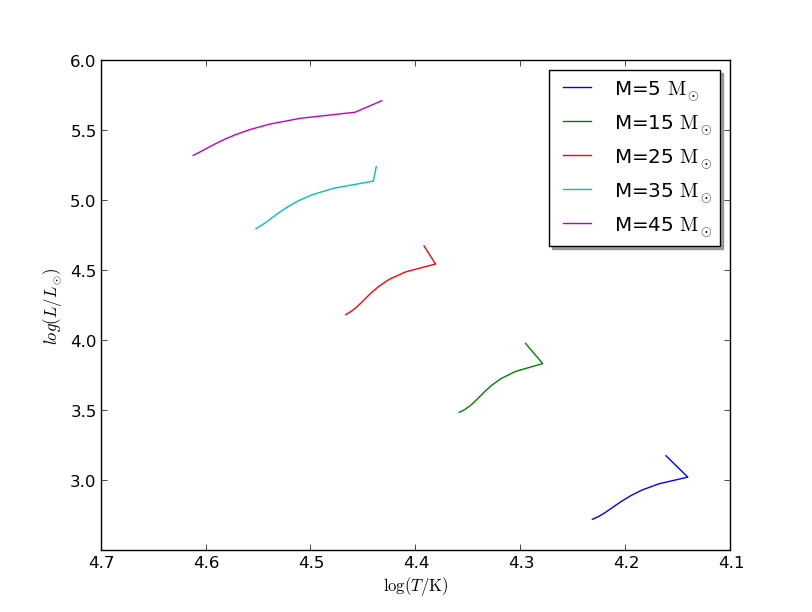
\includegraphics[width=\textwidth]{lumiradius}
  \caption{HRD for five different stars on their main sequence based on the evolutionary model of \citet{2000MNRAS.315..543H} \label{lumiradius}}
 \end{figure}
 
 The program does allow for freely changeable metalicities. For my purposes I use Z=0.02 for all stars to simulate
 a metalicity similar to that of our galactic neighborhood.\\
 I now run this model for every possible mass-age tuple and save the results in a matrix. This way I don't have to call the program for
 every distance-mass-age triple and massively cut down on computing time.\\
 After running the model I now know distance, mass, age, fractional main sequence age, luminosity and radius for any given star. I can now 
 use these informations to compute the apparent magnitudes.
 
 \begin{equation}
  M_{V}=V-5\cdot\log_{10}(r)+5-\mathrm{Red}
  \label{MV}
 \end{equation}
 
 \begin{equation}
  M_{bol}=M_{V}+BC
  \label{Mbol}
 \end{equation}
 
 \begin{equation}
  \frac{L}{L_\odot}=0.4\cdot(4.72-M_{bol})
  \label{LMbol}
 \end{equation}
 
 Where $M_{V}$ is the absolute visual magnitude, Red is the reddening as a function of r, $M_{bol}$ is the absolute bolometric 
 magnitude and BC is the Bolometric Correction. Using equations \ref{MV}, \ref{Mbol} and \ref{LMbol} I can now compute the apparent visual
 magnitude V:
 
 \begin{equation}
  V=5\cdot\log_{10}(r)-5+\mathrm{Red}+4.72-\frac{L}{L_\odot\cdot0.4}-BC
 \end{equation}
 
 To get a rough approximation for reddening, I use \citet*[Figure 9]{2005AJ....130..659A} pick three values and interpolate.\\
 The next thing I need to know are the probability densities for stars in space $\left(\frac{dp}{dV}\right)$, mass 
 $\left(\frac{dp}{dm}\right)$ and age $\left(\frac{dp}{dt}\right)$. In my simulation I assume a homogenous distribution of stars. 
 This makes finding a probability density for space very easy. Because of the radial symmetry of my problem the distribution becomes
 solely dependant on the distance from earth:
 
 \begin{equation}
  \frac{dp}{dV}=\frac{1}{V_{tot}}=\frac{1}{\frac43\cdot\pi\cdot r_{max}^3}
  \label{dpdV}
 \end{equation}
 
 I assume a constant star formation rate, so the probability density in age would be $\frac{dp}{dt}=\frac{1}{t_{ms}}$. I do however 
 use a logarithmic binning in age. Thus I can not simply use $\frac{dp}{dt}$ but instead need to find $\frac{dp}{d\log t}$ using the following 
 relation $d\log t=\frac{dt}{t \ln 10}$: 

 \begin{equation}
  \frac{dp}{d\log t}=\frac{t\ln 10}{t_{ms}}
 \end{equation}
 
 I also assume, that the stars are distributed in mass following the Salpeter IMF:
 $\frac{dp}{dM}=A\cdot M^{-2.35}$ \citep*{1955ApJ...121..161S}. Similar
 to the density function in age, I need to convert it for my logarithmic binning using $dlogM = \frac{dM}{M\ln 10}$
 
 \begin{equation}
  \frac{dp}{d\log M}=\ln 10 \cdot A\cdot M^{-1.35}
 \end{equation}
 
 Where A is a normalization factor, that needs to be computed. 
 
 \begin{equation}
  1=\int_{M_{min}}^{M_{max}}A\cdot M^{-2.35} dM =\left[ -1.35\cdot A\cdot M^{-1.35}\right]_{M_{min}}^{M_{max}}
 \end{equation}
 
 \begin{equation}
  A= \frac{1.35}{M_{min}^{-1.35}-M_{max}^{-1.35}}
 \end{equation}
 
 With this information I can now formulate an overarching probability density function with regard to $\tau$
 
 \begin{equation}
  \frac{dp}{d\tau}=\frac{dp}{dV}dV \cdot \frac{dp}{d\log t}d\log t \cdot \frac{dp}{d\log M}d\log M\cdot \frac{1}{d\tau}
 \end{equation}
 
 I now split $\tau$ in 20 bins. For every possible star in my sample I will check $\tau\le 1$ and $V\le 9$ This way I count every
 star on the main sequence, that falls below my magnitude cut. 
 
 \newpage
 \section{Tests}
 I conducted a few tests to see, whether my program makes sense. The most prominent I will explain in detail:
 
  \begin{figure}[h!]
  \begin{minipage}{0.49\textwidth}
   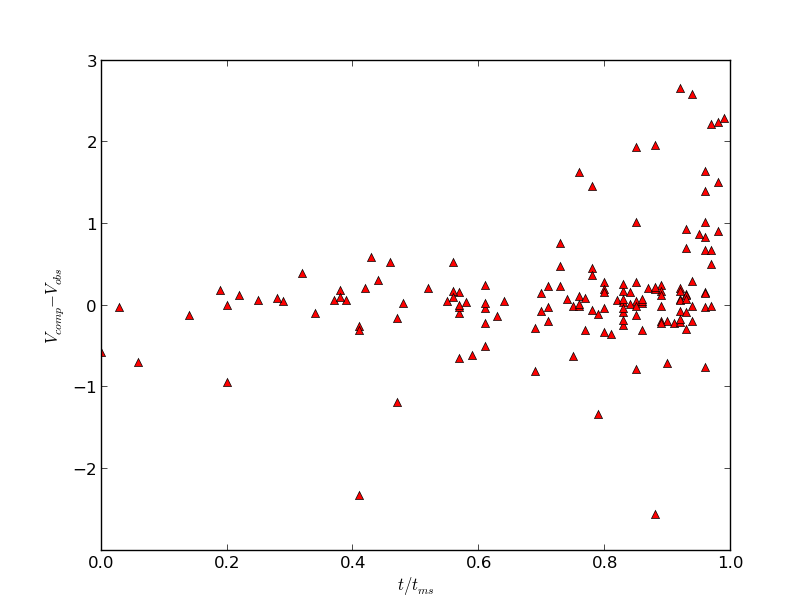
\includegraphics[width=\textwidth]{diffmagfracms}
  \end{minipage}
  \begin{minipage}{0.49\textwidth}
   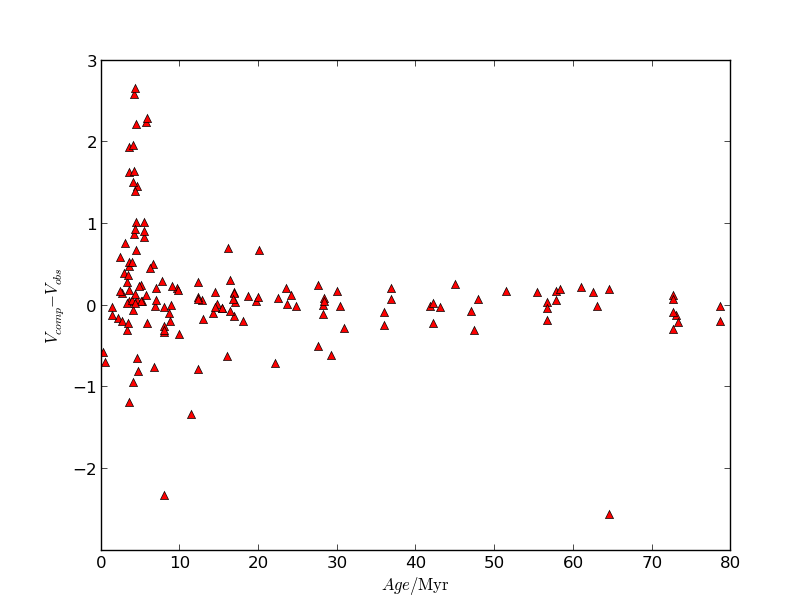
\includegraphics[width=\textwidth]{diffmagAge}
  \end{minipage}
  \begin{minipage}{0.49\textwidth}
   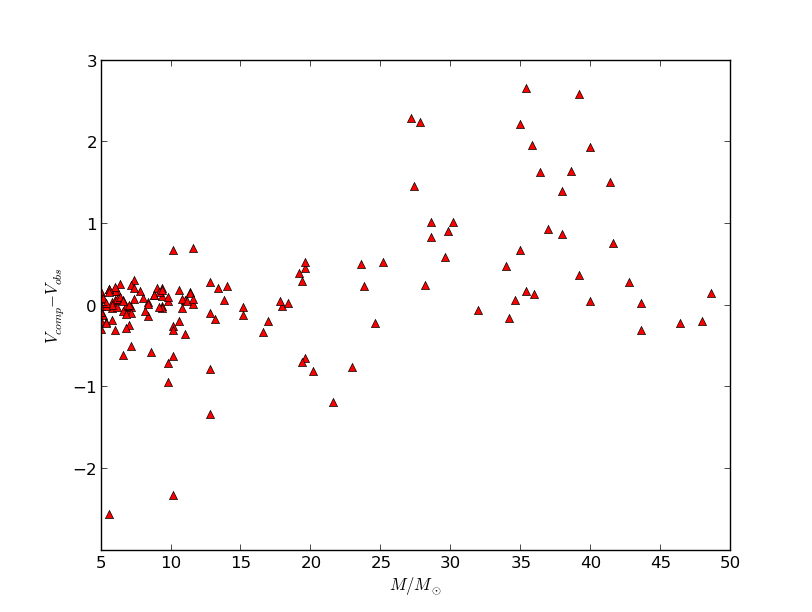
\includegraphics[width=\textwidth]{diffmagmass}
  \end{minipage}
  \begin{minipage}{0.49\textwidth}
   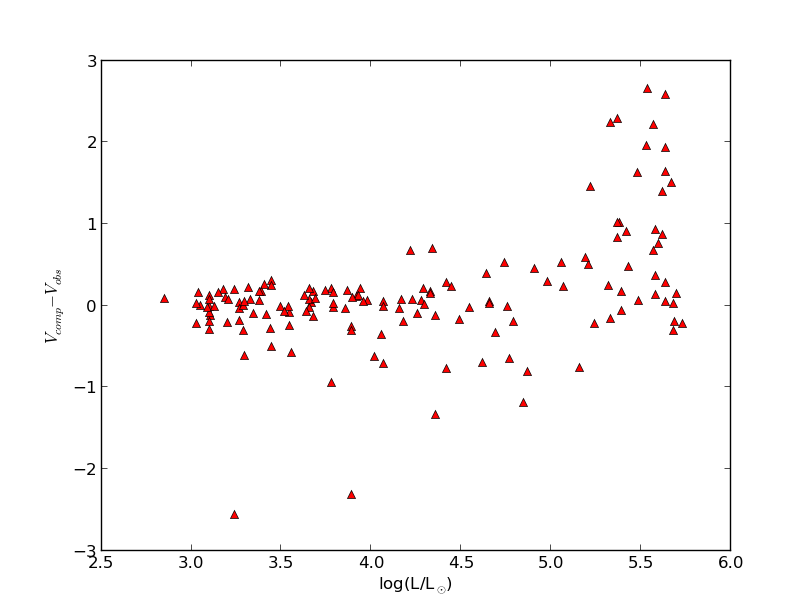
\includegraphics[width=\textwidth]{diffmaglogL}
  \end{minipage}
 \caption{Difference between computed and observed magnitudes as a function of fractional main sequence age (top left), total age
 (top right), Mass (bottom left) and $log_{10}(r/\mathrm{kpc})$ (bottom right). 
 The theoretical magnitudes ($V_{comp}$) were computed using stellar radius, luminosity and distance. The observational magnitudes ($V_{obs}$)
 were taken from a sample of 150 stars in the solar neighborhood between M=5M$_\odot$ and M=48M$_\odot$ \label{diffmag}}
 \end{figure}
 
 Figure \ref{diffmag} shows the difference between computed and observed magnitudes as a function of fractional main sequence age (top left),
 total age (top right), Mass (bottom left) and $log_{10}(\mathrm{L}/\mathrm{L}_\odot)$ (bottom right). \\
 The top graphs show, that there is a high offset to higher $V_{comp}$ at high $\tau$ and low absolute ages. This implies, that this 
 disagreement shows up in high mass stars near TAMS. This can be explained using \citep[figure 1]{2014A&A...570L..13C}. My code uses
 an evolutionary model similar to the one used on the lefthand side. $V_{obs}$ however is obtained using a model similar to the righthand
 side. The right model accounts for convective overshooting to a higher degree and thus the lifetime of a star is expanded. This agrees
 with the graph at the bottom left. The very high deviations are only seen in stars of Mass between $M=25M_\odot$ and $M\approx43M_\odot$.
 The convective overshooting, which extends the life of stars in the righthand side can explain for minor deviations. The massive differences
 between $M=25M_\odot$ and $M\approx 43M_\odot$ can be explained by taking into account inflation however. Near TAMS on the
 main sequence massive stars will undergo an expansion of their envelopes, thus increasing their surface area and subsequently their apparent
 magnitude. The right model takes this into account, whereas the left one 
 does not. For stars with a metalicity similar to the one in the solar neighborhood this effect occurs roughly at luminosities upwards of 
 $log(L/L_\odot)=5.3$, which is in perfect agreement with the graph on the bottom right.
 
 
 The deviation to negative values is mostly caused by extinction. It is most prevalent in lower absolute ages. 
 Stars of lower ages are primarily found in regions of active star formation. This would mean, that they are found in regions
 of high gas density. This gas will cause extinction and thus increase $V_{obs}$. My model for extinction does not take into account 
 these density fluctuations.
 
 
 \begin{figure}[h!]
  \begin{minipage}{0.49\textwidth}
   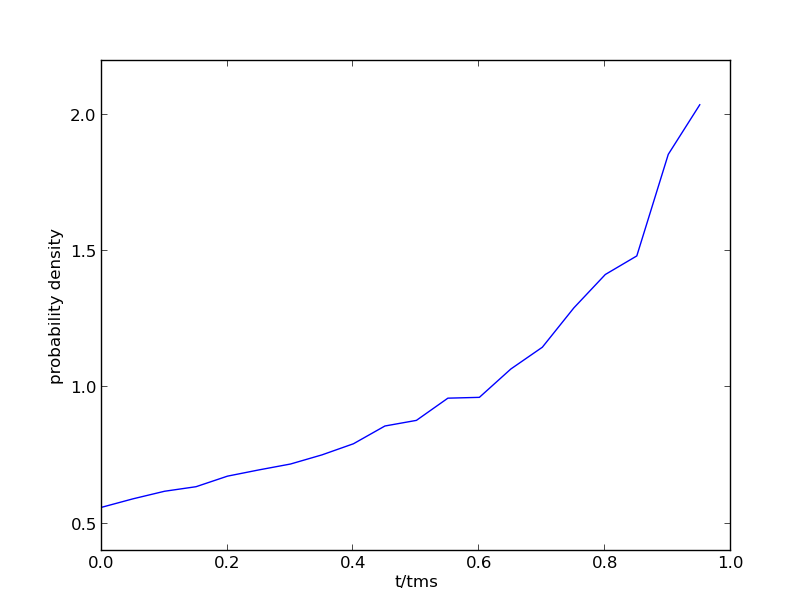
\includegraphics[width=\textwidth]{100-100-100}
  \end{minipage}
  \begin{minipage}{0.49\textwidth}
   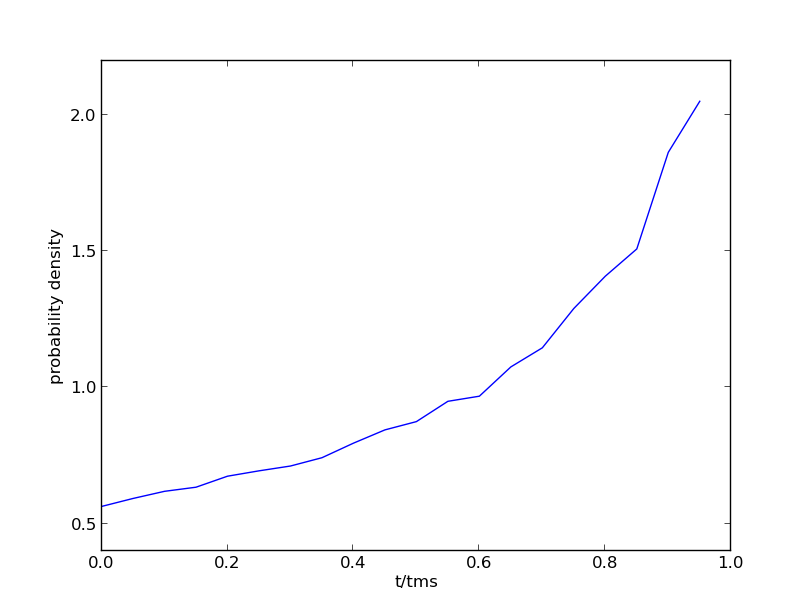
\includegraphics[width=\textwidth]{10-100-100}
  \end{minipage}
  \begin{minipage}{0.49\textwidth}
   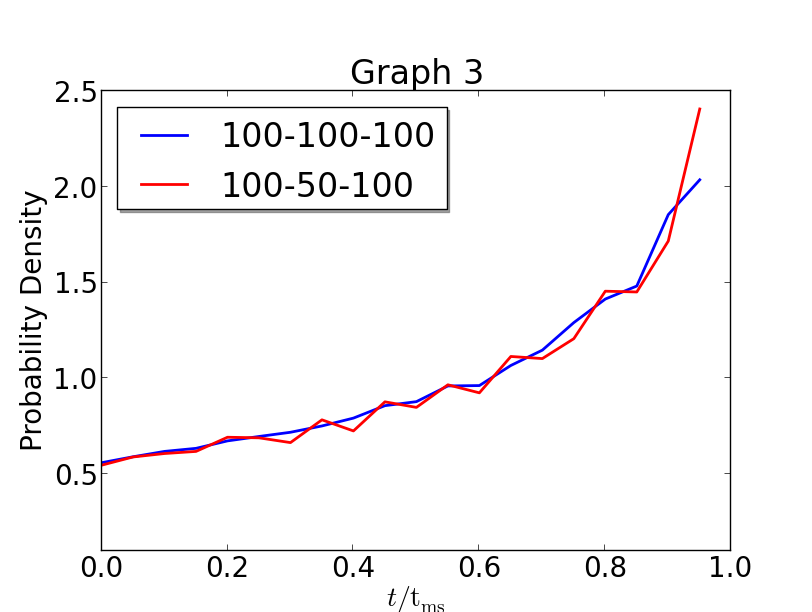
\includegraphics[width=\textwidth]{100-50-100}
  \end{minipage}
  \begin{minipage}{0.49\textwidth}
   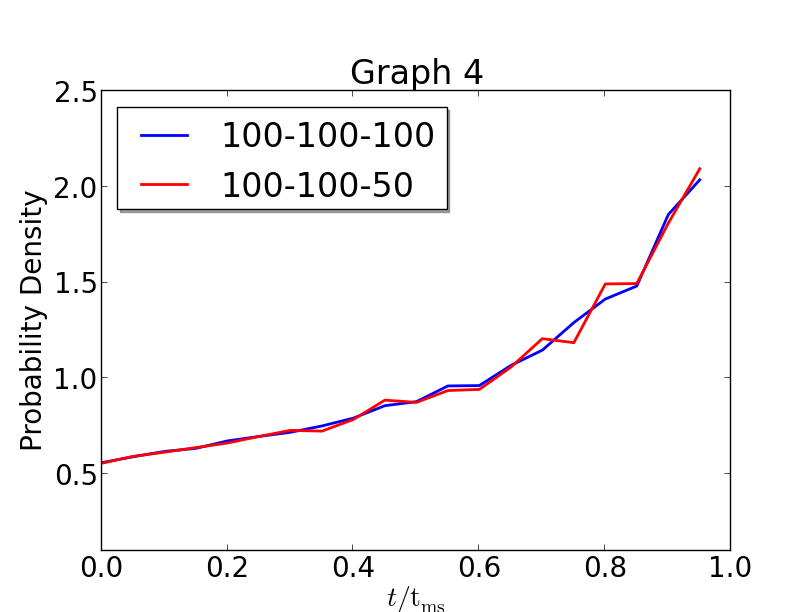
\includegraphics[width=\textwidth]{100-100-50}
  \end{minipage}
   \caption{Probability density function for all stars in my sample with a magnitude cut at V=9 with binnings of 100-100-100 (top left) 
   10-100-100 (top right) 100-50-100 (bottom left) and 100-100-50 (bottom right) in distance-mass-age.\label{binnings}}   
 \end{figure}
 
  Figure \ref{binnings} shows the probability density function for all stars in the sample
  with a magnitude cut at V=9 with different distance-mass-age binnings. The top left graph shows the reference graph
  with a binning of 100 for all variables. For the graph on the top right I reduced the binning in distance by a factor of ten. Both graphs
  are very similar. This means, that distance will be very robust to low binnings. \\
  The bottom two show the same function with the binning in mass (left) and age (right) halved. Here the discrepancies are very obvious. 
  Because of this I use a binning of 100-1000-1000 for my final data.
 
 \newpage
 \section{Results}
 \begin{figure}[h!]
   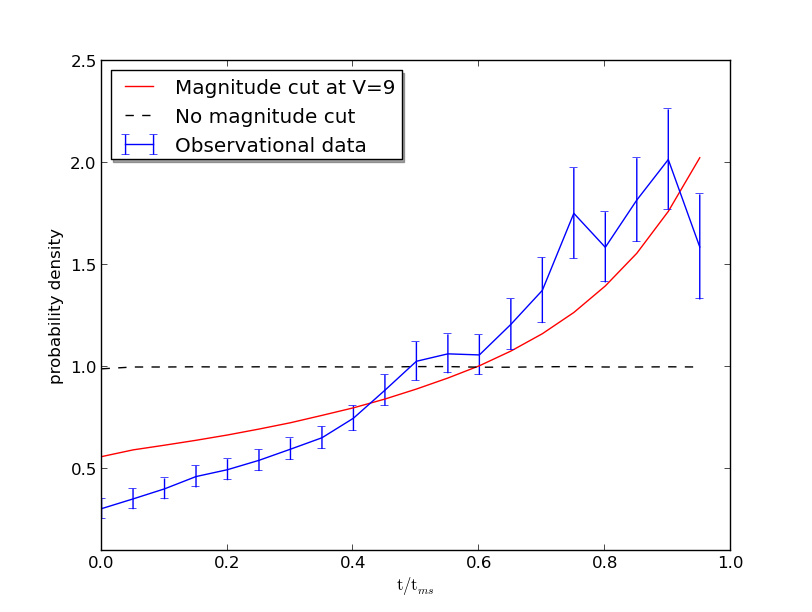
\includegraphics[width=\textwidth]{plot1}
   \caption{Probability density function with magnitude cut at V=9 (red line), probability density function without magnitude cut
   (black line) and observational data with error bars (blue line). All computed Data is obtained using a binning of 100-1000-1000
   in distance-mass-age. The observational data is taken from \textbf{citation?}\label{all3}}
 \end{figure}
 
 Figure \ref{all3} shows the probability density function with magnitude cut at V=9 (red line), probability density function without 
 magnitude cut (black line) and observational data with error bars (blue line).\\
 The probability density function without a magnitude cut shows, that the stars are uniformly distributed in $\tau$.\\
 The blue line seems to have a higher slope, than the red line. They do however compare pretty well 
 considering the program is only a minimalistic model. There are a lot of things, that can still be implemented:\\
 \begin{itemize}
  \item Right now the stars are distributed homogenously in a sphere of a 3kpc radius. To make it more accurate one could model our
  galactic neighborhood. Namely take into account the thickness of the galactic disk, which is smaller, than 3kpc.
  \item The program does not take into account binary stars. 
  \item From observations we know, that we live in a part of the galaxy with little star formation.  
  The density of young open starclusters increases the farther you move away from the solar system. As seen in Figure \ref{clusters}.
  \item My model for reddening is very approximated. It does not take into account density fluctuations in the interstellar medium. 
  The effects of which can be seen in figure \ref{diffmag}.
 \end{itemize}
 \begin{figure}[h!]
  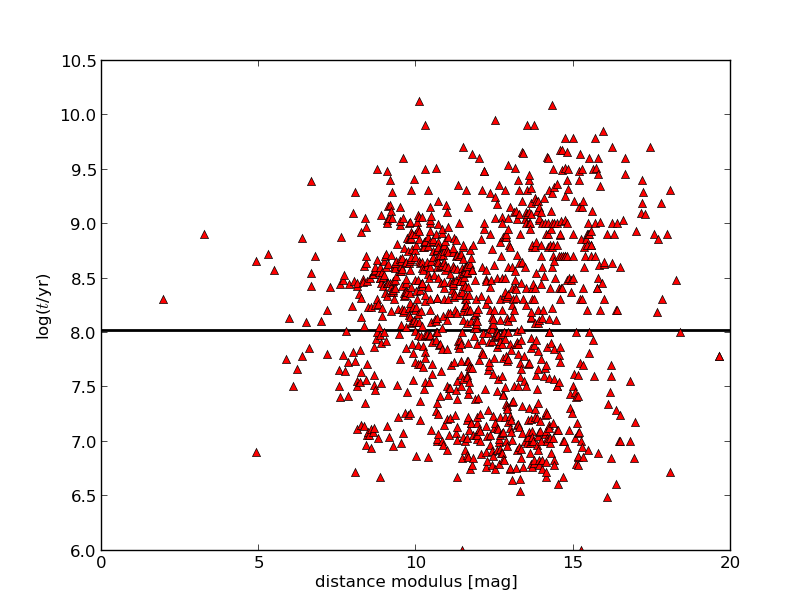
\includegraphics[width=\textwidth]{clusters}
  \caption{Open starclusters in our galaxy with distance modulus vs log(Age/yr)  \label{clusters}}
 \end{figure}

 
 \section{Conclusions}
 
 
 
 \bibliography{adssample}
\end{document}
